\documentclass[onecolumn, 12pt]{book}

\usepackage[latin1]{inputenc}   
\usepackage{amsmath}
\usepackage{algorithm}
\usepackage{algorithmic} 
%\usepackage[T1]{fontenc}

%\usepackage[francais]{babel}     
\usepackage{layout}    
\usepackage[top=2cm, bottom=2cm, left=2cm, right=2cm]{geometry} 
\usepackage{setspace}
\usepackage{soul}
\usepackage{color} 
\usepackage{verbatim}
\usepackage{moreverb}
\usepackage{listings}
\usepackage{url}
\usepackage{graphicx}
%\usepackage{epstopdf}
\usepackage[outdir=/home/willy/Documents/latexDoc/redaction/fusion_fichiers/images_fusionChapitres/]{epstopdf}
%\usepackage[outdir=./../../fusion_fichiers/images_fusionChapitres/]{epstopdf}
%\usepackage[outdir=./]{epstopdf}
\usepackage{caption}
\usepackage{setspace}
\usepackage{amsthm} % a ajouter dans le fichier simulations ou line graphes  => ne sert a rien amsmath
 
 
\title{Section : Graphes Iourtes}
\author{Wilfried Ehounou}
\date{\oldstylenums{\today}} 

\newtheorem{definition}{D\'efinition}
\newtheorem{theorem}{Theor\^eme}
\newtheorem{property}{Propri\'et\'e}
\newtheorem{claim}[theorem]{Claim}
\newtheorem{proposition}[theorem]{Proposition}
\newtheorem{lemma}[theorem]{Lemma}
\newtheorem{corollary}[theorem]{Corollary}
\newtheorem{conjecture}[theorem]{Conjecture}
\newtheorem{observation}{Observation}
\newtheorem{example}{Exemple}
\newtheorem{remark}{Remark}

%---- path figures ----
\graphicspath{
{/home/willy/Documents/latexDoc/redaction/fusion_fichiers/images_fusionChapitres/}
}
 
\begin{document}
\maketitle
\tableofcontents

\section{Graphes Iourtes}
Nous \'evaluons les performances de l'algorithme de correction sur des graphes dont les sommets ne sont couverts par aucune clique. Dans l'algorithme de couverture, ces sommets sont labellis\'es \`a $cliq(v) = -1$. Ces graphes sont dits {\em iourtes}.

\begin{figure}[htb!] 
\centering
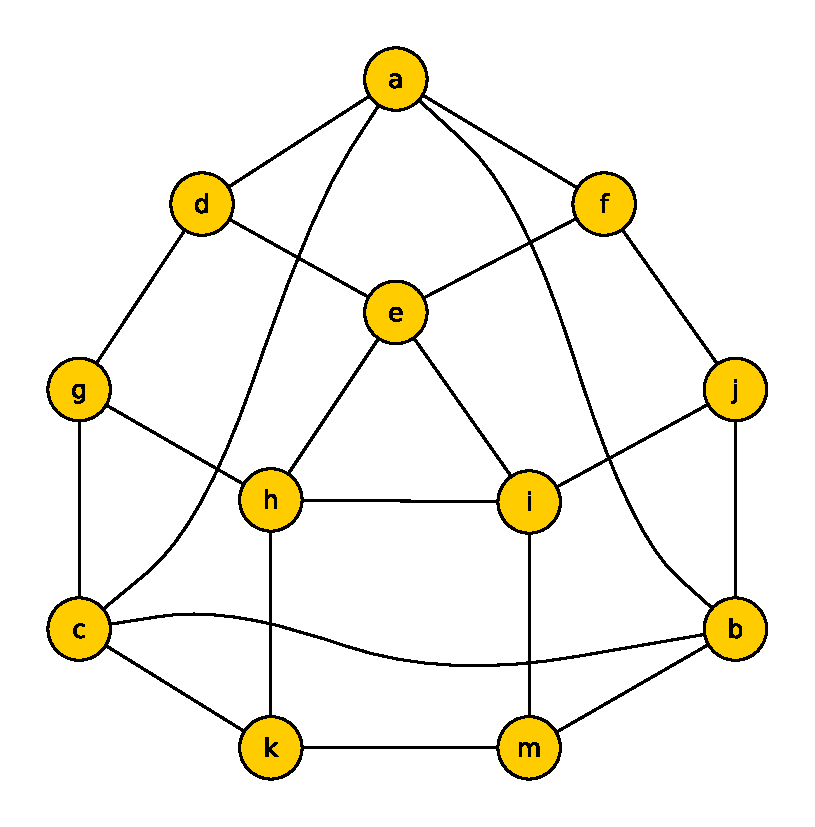
\includegraphics[scale=0.50]{grapheIourteG0.eps}
\caption{Graphe iourte $G_0 $}
\label{grapheIourteG0} 
\end{figure}

\begin{definition}
Un graphe iourte $G_0 = (V, E)$ est un graphe dont
\begin{itemize}
	\item l'ensemble $V$ contient $12$ sommets et l'ensemble $E$ a $21$ ar\^etes ($|V| = 12, |E| = 21)$.
	\item soit $N(v)$ l'ensemble des sommets adjacents \`a $v$. 
		les sommets $N(v)$ ne forment pas de cliques. \newline
		$\forall v \in V, \forall u, u' \in N(v),  (u, v) \in E \hspace{1 em} et  \hspace{1 em} (u, u') \notin E $
	\item $G_0$ est {\em 4-r\'egulier}.
\end{itemize}
\end{definition}
La figure \ref{grapheIourteG0} est une illustration d'un graphe iourte $G_0$.
\newline
Soient $k$ la profondeur c'est-\`a-dire le nombre de fois qu'on modifie $G_0$ par la transformation d'ar\^etes en chaines de longueur $2$ et $G_0^k$ le graphe $G_0$ de profondeur $k$.

\begin{theorem}
Le graphe $G_0^k$ est un graphe iourte de $3k+12$ sommets et $6k + 21$ ar\^etes
\end{theorem} 

\begin{proof}
Nous distinguons trois sommets $A$, $B$, $C$ dans $G_0$. 
\`A partir de $G_0$, on obtient $G_0^1$ en ajoutant de $3$ sommets par les modifications  suivantes.
Nous remplacons chaque ar\^ete $[A,B]$, $[B,C]$,  $[A,C]$  par une chaine de longueur $2$. 
Les sommets ainsi cr\'ees deviennent les nouveaux sommets   $A$, $B$, $C$ qui forment un cycle de longueur $3$.
Ainsi le voisinage de ces $3$ sommets  ne peuvent pas \^etre couvert par une ou deux cliques.
En rep\'etant $k$ fois cette modification, nous obtenons le graphe $G_0^k$ de $3k+12$ sommets et $6k+21$ ar\^etes.
\end{proof}

La figure \ref{grapheIourteG01eExecution} d\'ecrit un line-graphe $L(G_0)$ couvrant $G_0$ en lui ajoutant $6$ ar\^etes (en pointill\'ees).
Ces $6$ ar\^etes d\'esignent la plus petite modification possible de $G_0$ en termes de co\^ut d'ajout et suppression.
Par cons\'equent $DL(G_0) = 6$. 
\begin{conjecture}
\label{conjectureDLIourte}
La distance line de $G_0^k$ v\'erifie $DL(G_0^k) \le 3k+6$.
\end{conjecture}
\begin{figure}[htb!] 
\centering
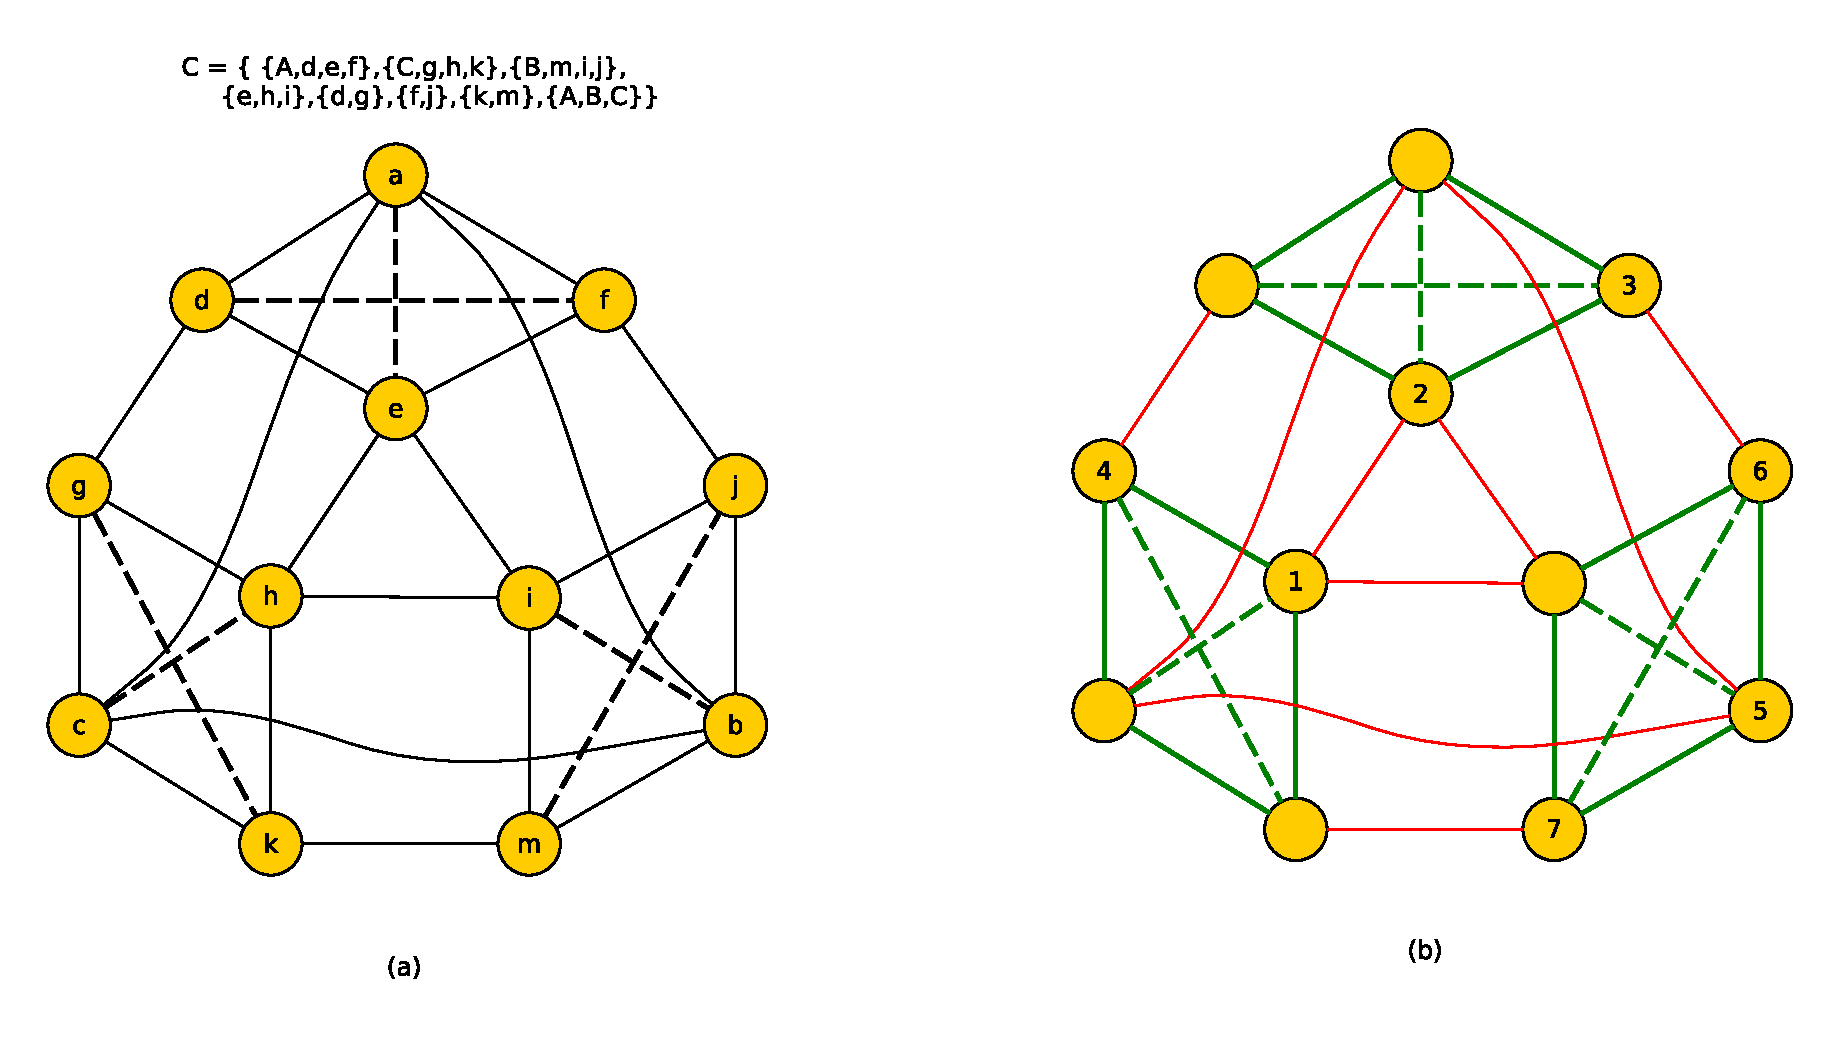
\includegraphics[scale=0.50]{grapheIourteG01eExecution.eps}
\caption{Une correction du graphe $G_0$ : $DL(G_0) = 6$ }
\label{grapheIourteG01eExecution} 
\end{figure}
Le line-graphe  $L(G_0^k)$ couvrant $G_0^k$ ayant une distance de Hamming de $3k+6$ s'obtient \`a partir de  $L(G_0^{k-1})$ en supprimant une ar\^ete parmi deux dans un cycle de taille $6$. Ce cycle est form\'e par les anciens sommets $A$, $B$, $C$ (de $G_0^{k-1}$) et les nouveaux sommets $A$, $B$, $C$ de $G_0^k$, soit une suppression de $3$.
Chaque ar\^ete non supprim\'ee dans ce cycle forme une clique de taille $2$ et  le nouveau cycle de taille $3$ entre les sommets $A$, $B$, $C$ forme une nouvelle clique (en rempla\c cant la pr\'ec\'edente clique de $L(G_0^{k-1})$).
\newline
Dans la section suivante, nous analysons les distances lines obtenues par l'algorithme de correction par rapport \`a la conjecture \ref{conjectureDLIourte}.

\subsection{Correction des graphes Iourtes}
Dans cette partie, nous v\'erifions que la correction de graphes iourtes de diff\'erentes profondeurs modifie $3k+6$ ar\^etes.
 En d'autres termes, nous \'etudions l'impact de l'ajout/suppression d'ar\^etes lors de la correction d'un sommet dans le processus de correction du graphe.
Pour ce faire, nous construisons $50$ graphes iourtes dont chaque graphe a une profondeur $k \in [0,50]$.
Sur chaque graphe $G_0^k$, nous ex\'ecutons  l'algorithme de correction  $50$ fois puis nous r\'ecup\'erons la distance de Hamming minimale entre $G_0^k$ et les line-graphes obtenus i.e la distance line.
\newline
Soient les fonctions de co\^ut  {\em ajouter une ar\^ete} $\phi^{+}(u,v)$ et {\em supprimer une ar\^ete} $\phi^{-}(u,v)$ avec $u,v \in V$.
Nous consid\'erons trois niveaux de priorit\'e :
\begin{itemize}
	\item aucune priorit\'e : l'ajout et la suppression d'une ar\^ete co\^utent $1$ ($\phi^{+} = \phi^{-} = 1$)
	\item priorit\'e ajout : ajouter une ar\^ete co\^ute $\phi^{+} = 1$ alors qu'en supprimer une co\^ute $\phi^{-} = 10$; 
	\item priorit\'e suppression : ajouter une ar\^ete co\^ute $\phi^{+} = 10$ alors qu'en supprimer une co\^ute $\phi^{-} = 1$; 
\end{itemize}
Les figures \ref{priorAjout1Ajout10}(a)  et \ref{priorAjout1Supp10}(a) contiennent trois courbes : la droite d'\'equation $y = 3k+6$ d\'esignant le comportement id\'eal de l'algorithme de correction, les courbes labellis\'ees {\em dl\_ajout\_X} et {\em dl\_supp\_Y}  repr\'esentant respectivement le comportement de la correction quand $\phi^{+} = X$ et $\phi^{-} = Y$ avec $X, Y \in \{1,10\}$. 
La courbe  {\em dl\_ajout\_X} d\'esigne la priorisation sur l'ajout d'ar\^etes en attribuant un poids $w\_ajout = 1$ pour l'ajout et un poids $w\_supp = X$ pour une suppression.
De m\^eme la  courbe  {\em dl\_supp\_Y} d\'esigne la priorisation sur la suppression d'ar\^etes en attribuant un poids $w\_supp = 1$ pour la suppression et un poids $w\_ajout = Y$ pour un ajout.

\paragraph{Correction en priorisant l'ajout d'ar\^etes} %\newline
\begin{figure}[htb!] 
\centering
\includegraphics[scale=0.250]{comparaison_prior_ajout_wi_1_ajout_wi_10_distance_line_vs_3k_6_graphe_iourte.jpeg}
\caption{(a)Priorisation sur l'ajout d'ar\^etes : la courbe {\em dl\_ajout\_1} est la priorisation sur l'ajout d'ar\^etes avec un poids $w\_ajout=1$ pour l'ajout et $w\_supp = 1$ pour la suppression,   la courbe {\em dl\_ajout\_10} est la priorisation sur l'ajout d'ar\^etes avec un poids $w\_ajout=1$ pour l'ajout et $w\_supp = 10$ pour la suppression, (b) taux de suppression d'ar\^etes de $G_0^k$ pour les priorisations  {\em dl\_ajout\_1} et  {\em dl\_ajout\_10}, (c) la diff\'erence de distances lines entre les priorisations {\em dl\_ajout\_1} et  {\em dl\_ajout\_10}  et la droite $y=3k+6$.  }
\label{priorAjout1Ajout10} 
\end{figure}
L'exemple th\'eorique effectu\'e sur le graphe $G_0$ propose la distance de Hamming minimale $DL= 6$ en n'ajoutant que des ar\^etes (voir figure \ref{grapheIourteG01eExecution}).
Nous allons prioriseralors  l'ajout des ar\^etes dans la correction c'est-\`a-dire attribuer des poids \'elev\'es  $w\_supp = 10$ pour la suppression et des poids faibles $w\_ajout = 1$ pour l'ajout d'ar\^etes. Cette priorisation est repr\'esent\'ee par la courbe {\em dl\_ajout\_10} et nous comparons  cette courbe  avec la courbe {\em dl\_ajout\_1}( $w_{supp} = w_{ajout} = 1$).
\newline
Les courbes {\em dl\_ajout\_1} et {\em dl\_ajout\_10} \'evoluent  lin\'eairement avec des pentes respectives de ($\alpha_{dl\_ajout\_1} \approx 3.76$ et $\alpha_{dl\_ajout\_10} \approx 4.96$).
La courbe {\em dl\_ajout\_1} croit faiblement par rapport \`a celle de {\em dl\_ajout\_10}.
De m\^eme, l'\'ecart des distances line entre les courbes {\em dl\_ajout\_1} et $y=3k+6$ croit lin\'eairement alors que celui entre les courbes {\em dl\_ajout\_10} et $y=3k+6$ est une succession de croissance et de decroissance (voir figure \ref{priorAjout1Ajout10}(c)). 
Cette d\'ecroissance constat\'ee \`a $k=\{6,20,26,36,42\}$ correspond \`a l'ajout de peu d'ar\^etes (extremums inf\'erieurs de la courbe {\em aretes\_G\_k\_notIn\_LG\_ajout\_10} de la figure \ref{priorAjout1Ajout10}(b)) dans les graphes $G_0^k$.
 Il se deduit que la courbe {\em dl\_ajout\_10} ajoute beaucoup d'ar\^etes dans $G_0^k$ par rapport \`a la courbe  {\em dl\_ajout\_1}. 
Ce qui est normal puisque l'hypoth\`ese de depart est la priorisation de l'ajout d'ar\^etes. 
Toutefois, en observant la figure \ref{priorAjout1Ajout10}(b), on remarque que {\em dl\_ajout\_10} supprime moins d'ar\^etes dans $G_0^k$ par rapport \`a {\em dl\_ajout\_1}.
Le fait que  l'ajout et la suppression dans {\em dl\_ajout\_1} ont le m\^eme co\^ut ($\phi^{+} = \phi^{-} = 1$) explique ces suppressions massives et ces suppressions engendrent de nombreux ajouts d'ar\^etes pour obtenir un line-graphe connexe.
\newline
La priorisation sur l'ajout d'ar\^etes donne de mauvais r\'esultats parce que la courbe {\em dl\_ajout\_10} est tr\`es \'eloign\'e de celle de $y = 3k+6$ lorsque $k$ grandit.
Par ailleurs, ne priviliger aucune priorisation donne de bons r\'esultats car l'\'ecart entre {\em dl\_ajout\_1} et $y=3k+6$ est  faible pour $k \le 8$ et au d\'el\`a croit lin\'eairement mais faiblement  \ref{priorAjout1Ajout10}(c). Et cela decoule de l'ajout des ar\^etes dans $G_0^k$ pour des lines-graphes $L(G_0^k)$.  
\newline
Puisque prioriser l'ajout d'ar\^etes ne produit pas de bonnes r\'esultats, que se passe-t-il si on priorise la suppression?   


%La courbe {\em dl\_ajout\_1} croit faiblement alors que la courbe {\em dl\_ajout\_10}  croit fortement et l'\'ecart entre ces deux courbes \'evolue lin\'eairement.
%La courbe  {\em dl\_ajout\_10} supprime moins d'ar\^etes de $G_0^k$ que celle {\em dl\_ajout\_1} comme nous le constatons sur la figure \ref{priorAjout1Ajout10}(b) o\`u le taux de suppressions de {\em dl\_ajout\_1} est sup\'erieure \`a celui de {\em dl\_ajout\_10}. Cela s'explique par le fait que l'ajout et la suppression dans {\em dl\_ajout\_1} ont leur meme co\^ut ($\phi^{+} = \phi^{-} = 1$) et la correction tend \`a supprimer les ar\^etes. En plus la courbe {\em dl\_ajout\_10} ajoute plus d'ar\^etes dans $G_0^k$ que  celle {\em dl\_ajout\_1}.
%\newline
%La priorisation sur l'ajout d'ar\^etes donne de mauvais r\'esultats parce que l'\'ecart entre les courbes {\em dl\_ajout\_10} et $y=3k+6$ croit lin\'eairement lorsque $k$ grandit.
%Par ailleurs ne priviliger aucune priorisation a de bons r\'esultats car l'ecart entre {\em dl\_ajout\_1} et $y=3k+6$ croit faiblement \`a cause de la suppression des ar\^etes de $G_0^k$ et du faible ajout dans les lines graphes $L(G_0^k)$.
%\newline 
%Puisque prioriser l'ajout d'ar\^etes ne produit pas de bonnes r\'esultats, que ce passe-t-il si on priorise la suppression?   



\paragraph{Correction en priorisant la suppression d'ar\^etes } %\newline
\begin{figure}[htb!] 
\centering
\includegraphics[scale=0.250]{comparaison_prior_ajout_wi_1_supp_wi_10_distance_line_vs_3k_6_graphe_iourte.jpeg}
\caption{(a)Priorisation sur la suppression d'ar\^etes : la courbe {\em dl\_supp\_10} est la priorisation sur la suppression d'ar\^etes avec un poids $w\_supp=1$ \`a la suppression et $w\_ajout = 10$ \`a l'ajout,   la courbe {\em dl\_ajout\_1} est la priorisation sur l'ajout d'ar\^etes avec un poids $w\_ajout=1$ pour l'ajout et $w\_supp = 1$ pour la suppression, (b) taux de suppression d'ar\^etes de $G_0^k$, (c) la diff\'erence de distances lines entre les priorisations {\em dl\_ajout\_1} et  {\em dl\_supp\_10}  et la droite $y=3k+6$. }
\label{priorAjout1Supp10} 
\end{figure}
Puisque ajouter et supprimer au m\^eme co\^ut produit de bons r\'esultats pour les distances-line,  nous attribuons des poids \'elev\'es  $w\_ajout = 10$ pour l'ajout et des poids faibles $w\_supp = 1$ pour la suppression d'ar\^etes. La courbe repr\'esentant cette priorisation est  {\em dl\_supp\_10} et nous la comparons avec la courbe $dl\_ajout\_1$.
\newline
Dans la figure  \ref{priorAjout1Supp10}(a), les courbes {\em dl\_ajout\_1} et {\em dl\_supp\_10} sont confondues jusqu'\`a la profondeur $k \le 20$ et au d\'el\`a de $k > 20$, il existe un leger \'ecart entre ces deux courbes. Nous l'expliquons par leurs pentes tr\`es proches ($\alpha_{dl\_ajout\_1} \approx 3.93$ et $\alpha_{dl\_supp\_10} \approx 3.78$) qui accentuent l'\'ecart des distances-line quand $k$ croit (voir figure \ref{priorAjout1Supp10}(c)). 
Cet \'ecart est caus\'e par la suppression d'ar\^etes car {\em dl\_supp\_10} supprime environ $50\%$ des ar\^etes de $G_0^k$ alors que  {\em dl\_ajout\_1} en supprime environ $45\%$ (voir figure \ref{priorAjout1Supp10}(b)).
Toutefois, la courbe {\em dl\_supp\_10} donne de meilleurs r\'esultats pour $k > 22$ puisque {\em dl\_supp\_10} se rapproche de $y=3k+6$ (voir figure \ref{priorAjout1Supp10}(c)).


Nous pouvons conclure que la meilleure m\'ethode de correction des graphes iourtes est la priorisation de la suppression d'ar\^etes.
Cependant la conjecture \ref{conjectureDLIourte} ne se v\'erifie pas parce que certaines ar\^etes de $G_0^k$ ont \'et\'e supprim\'ees du line-graphe $L(G_0^k)$ et ce taux de suppression de ces ar\^etes  avoisine les $50\%$.

%\paragraph{Correction sans priorit\'e} %\newline
%\begin{figure}[htb!] 
%\centering
%%\includegraphics[scale=0.250]{comparaison_prior_ajout_wi_1_supp_wi_1_distance_line_vs_3k_6_graphe_iourte.jpeg}
%\caption{}
%\label{priorAjout1Supp1} 
%\end{figure}
%Ces deux courbes \'evoluent identiquement parce que elles ont les m\^emes co\^uts et la m\^eme pente ($\alpha_{dl\_ajout\_1} \approx $ et $\alpha_{dl\_supp\_1} \approx $). 
%\newline
%Par ailleurs, la pente de la courbe $y = 3k+6$ est $\alpha_{3k+6} = $. Ce qui explique la forte croissante des courbes {\em dl\_ajout\_1} et {\em dl\_supp\_1} par rapport \`a celle $y = 3k+6$.
%Les ordonn\'es \`a l'origine des courbes $y = 3k+6$, {\em dl\_ajout\_1} et {\em dl\_supp\_1} sont $6$, $7$ et $8$ et L' \'ecart entre leurs distances line croit lin\'eairement.
%Nous avons remarqu\'e que l'algorithme supprime des ar\^etes de $G_0^k$ l'obligeant \`a ajouter des ar\^etes suppl\'ementaires pour obtenir un line-graphe. Ce qui explique les diff\'erences entre les ordonn\'ees \`a l'origine et la croissante lin\'eaire de l'\'ecart.
%\newline
%Ayant constat\'e que la correction supprimait des ar\^etes de $G_0^k$ et en ajouter d'autres, nous allons imposer \`a l'algorithme de supprimer peu d'ar\^etes de base dans le paragraphe suivant.
%
%%%% a exploiter ds un autre paragraphe
%Nous remarquons que les courbes {\em dl\_ajout\_1} et {\em dl\_supp\_10} sont confondues jusqu'\`a la profondeur $k \le 20$ et au d\'el\`a de $k > 20$, il existe un leger \'ecart entre ces deux courbes. Nous l'expliquons par leurs pentes tr\`es proches ($\alpha_{dl\_ajout\_1} \approx $ et $\alpha_{dl\_supp\_10} \approx $) qui accentuent l'\'ecart quand $k$ croit.



\end{document}

